\documentclass{beamer}
\usetheme{Berlin} 
\usecolortheme{dolphin}
\usefonttheme{structuresmallcapsserif}
%\usecolortheme[named=Brown]{structure}
\usepackage{algorithmic}
\usepackage{listings}
%\usepackage{beamerthemesplit}
\usepackage{amsfonts,amssymb}
\usepackage[croatian]{babel}
\usepackage{color}
\usepackage[utf8]{inputenc}

\title{Q Learning}
\author{Ivan Androš \\ Dejan Peretin \\ Petra Podolski}
\date{25. svibnja 2011.}

\begin{document}

\frame{\titlepage} 

\section{Uvod}
\frame{
\frametitle{Q Learning}
\begin{itemize}
\item
Tehnika učenja s podrškom.
\item
Agent uči evaluacijsku funkciju
$$Q:S\times A \to \mathbb{R}$$
gdje je $S$ skup stanja, a $A$ skup akcija akcija.
\item 
Agentu ne mora biti poznat model okoliša.
\end{itemize}
}

\section{Primjer problema}
\frame{
	\frametitle{Kretanje robota}
\begin{figure}
	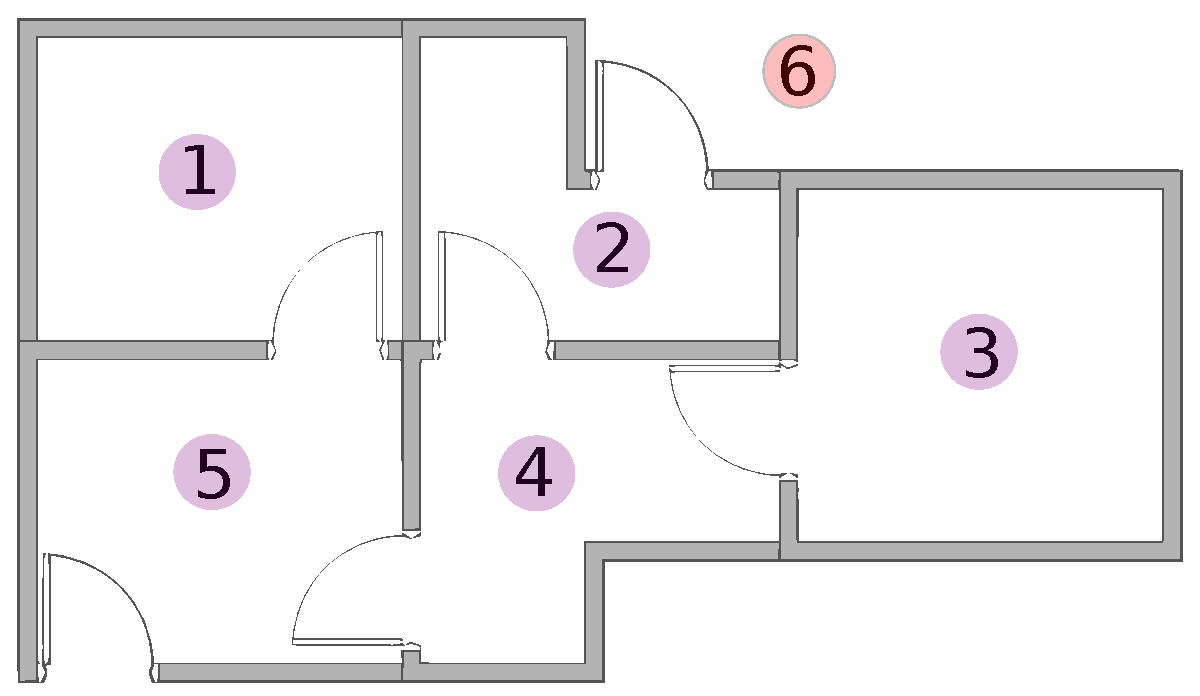
\includegraphics[scale=0.5]{slike/soba.pdf}
	\caption{Agent se nalazi u jednoj od soba, mora izaći van}
\end{figure}
	
}

\frame{
\begin{figure}
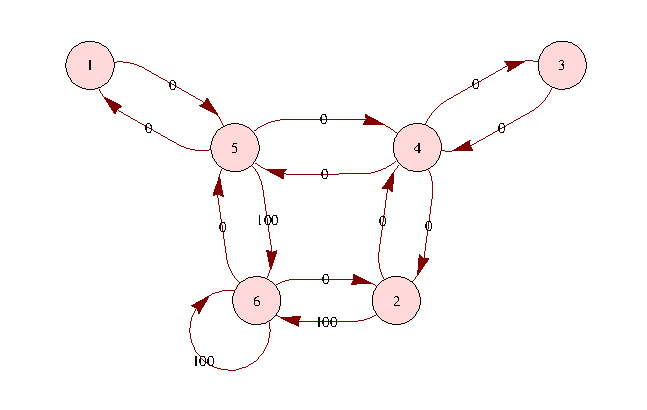
\includegraphics[scale=0.8]{slike/R.pdf}
	\caption{Dijagram stanja prethodnog tlocrta}
\end{figure}
}

\section{Opis algoritma}

\frame{
	\frametitle{Učenje funkcije $Q$}
	\begin{picture}(400,0)
		\put(0,0){
			\mbox{
				$R=
				\left[
				\begin{array}{cccccc}
				- & - & - & - & 0 & - \\
				- & - & - & 0 & - & 100 \\
				- & - & - & 0 & - & - \\
				- & 0 & 0 & - & 0 & - \\
				0 & - & - & 0 & - & 100 \\
				- & 0 & - & - & 0 & 100 \\
				\end{array}
				\right]\quad Q=
				\left[
				\begin{array}{cccccc}
				0 & 0 & 0 & 0 & 0 & 0 \\
				0 & 0 & 0 & 0 & 0 & 0 \\
				0 & 0 & 0 & 0 & 0 & 0 \\
				0 & 0 & 0 & 0 & 0 & 0 \\
				0 & 0 & 0 & 0 & 0 & 0 \\
				0 & 0 & 0 & 0 & 0 & 0 \\
				\end{array}
				\right]
				$
			}
		}
	\end{picture}

}
\frame{
	\frametitle{Učenje funkcije $Q$}
	\begin{picture}(400,0)
		\put(0,0){
			\mbox{
				$R=
				\left[
				\begin{array}{cccccc}
				- & - & - & - & 0 & - \\
				- & - & - & 0 & - & 100 \\
				- & - & - & 0 & - & - \\
				- & 0 & 0 & - & 0 & - \\
				0 & - & - & 0 & - & 100 \\
				- & 0 & - & - & 0 & 100 \\
				\end{array}
				\right]\quad Q=
				\left[
				\begin{array}{cccccc}
				0 & 0 & 0 & 0 & 0 & 0 \\
				0 & 0 & 0 & 0 & 0 & 0 \\
				0 & 0 & 0 & 0 & 0 & 0 \\
				0 & 0 & 0 & 0 & 0 & 0 \\
				0 & 0 & 0 & 0 & 0 & 0 \\
				0 & 0 & 0 & 0 & 0 & 0 \\
				\end{array}
				\right]
				$
			}
		}
	\put(10, 23){\vector(1,0){20}}
	\end{picture}

}
\frame{
\frametitle{Učenje funkcije $Q$}
	\begin{picture}(400,0)
		\put(0,0){
			\mbox{
				$R=
				\left[
				\begin{array}{cccccc}
				- & - & - & - & 0 & - \\
				- & - & - & 0 & - & {\color{red}100} \\
				- & - & - & 0 & - & - \\
				- & 0 & 0 & - & 0 & - \\
				0 & - & - & 0 & - & 100 \\
				- & 0 & - & - & 0 & 100 \\
				\end{array}
				\right]\quad Q=
				\left[
				\begin{array}{cccccc}
				0 & 0 & 0 & 0 & 0 & 0 \\
				0 & 0 & 0 & 0 & 0 & {\color{red}0} \\
				0 & 0 & 0 & 0 & 0 & 0 \\
				0 & 0 & 0 & 0 & 0 & 0 \\
				0 & 0 & 0 & 0 & 0 & 0 \\
				0 & 0 & 0 & 0 & 0 & 0 \\
				\end{array}
				\right]
				$
			}
		}
	\put(10, 23){\vector(1,0){20}}
	\end{picture}

}

\frame{
\frametitle{Učenje funkcije $Q$}
	\begin{picture}(400,0)
		\put(0,0){
			\mbox{
				$ R=
				\left[
				\begin{array}{cccccc}
				- & - & - & - & 0 & - \\
				- & - & - & 0 & - & {\color{red}100} \\
				- & - & - & 0 & - & - \\
				- & 0 & 0 & - & 0 & - \\
				0 & - & - & 0 & - & 100 \\
				- & 0 & - & - & 0 & 100 \\
				\end{array}
				\right]\quad Q=
				\left[
				\begin{array}{cccccc}
				0 & 0 & 0 & 0 & 0 & 0 \\
				0 & 0 & 0 & 0 & 0 & {\color{red}0} \\
				0 & 0 & 0 & 0 & 0 & 0 \\
				0 & 0 & 0 & 0 & 0 & 0 \\
				0 & 0 & 0 & 0 & 0 & 0 \\
				0 & 0 & 0 & 0 & 0 & 0 \\
				\end{array}
				\right]
				$
			}
		}
	\put(10, 23){\vector(1,0){20}}
	\put(10, -31){\vector(1,0){20}}
	\end{picture}

}
\frame{
\frametitle{Učenje funkcije $Q$}
	\begin{picture}(400,0)
		\put(0,0){
			\mbox{
				$R=
				\left[
				\begin{array}{cccccc}
				- & - & - & - & 0 & - \\
				- & - & - & 0 & - & {\color{red}100} \\
				- & - & - & 0 & - & - \\
				- & 0 & 0 & - & 0 & - \\
				0 & - & - & 0 & - & 100 \\
				- & {\color{red}0} & - & - & {\color{red}0} & {\color{red}100} \\
				\end{array}
				\right]\quad Q=
				\left[
				\begin{array}{cccccc}
				0 & 0 & 0 & 0 & 0 & 0 \\
				0 & 0 & 0 & 0 & 0 & {\color{red}0} \\
				0 & 0 & 0 & 0 & 0 & 0 \\
				0 & 0 & 0 & 0 & 0 & 0 \\
				0 & 0 & 0 & 0 & 0 & 0 \\
				0 & 0 & 0 & 0 & 0 & 0 \\
				\end{array}
				\right]
				$
			}
		}
	\put(10, 23){\vector(1,0){20}}
	\put(10, -31){\vector(1,0){20}}
	\end{picture}

}
\frame{
\frametitle{Učenje funkcije $Q$}
	\begin{picture}(400,0)
		\put(0,0){
			\mbox{
				$ R=
				\left[
				\begin{array}{cccccc}
				- & - & - & - & 0 & - \\
				- & - & - & 0 & - & {\color{red}100} \\
				- & - & - & 0 & - & - \\
				- & 0 & 0 & - & 0 & - \\
				0 & - & - & 0 & - & 100 \\
				- & {\color{red}0} & - & - & {\color{red}0} & {\color{red}100} \\
				\end{array}
				\right]\quad Q=
				\left[
				\begin{array}{cccccc}
				0 & 0 & 0 & 0 & 0 & 0 \\
				0 & 0 & 0 & 0 & 0 & {\color{red}0} \\
				0 & 0 & 0 & 0 & 0 & 0 \\
				0 & 0 & 0 & 0 & 0 & 0 \\
				0 & 0 & 0 & 0 & 0 & 0 \\
				0 & {\color{red}0} & 0 & 0 & {\color{red}0} & {\color{red}0} \\
				
				\end{array}
				\right]
				$
			}
		}
	\put(10, 23){\vector(1,0){20}}
	\put(10, -31){\vector(1,0){20}}
	\put(0,-60){
			\mbox{$
			Q_{2,6} = R_{2,6}+0.8 \cdot \max\{Q_{6,2},Q_{6,5},Q_{6,6}\}
			        = 100+0.8 \cdot 0
			        = 100
			$
			}}
	\end{picture}

}
\frame{
\frametitle{Učenje funkcije $Q$}
	\begin{picture}(400,0)
		\put(0,0){
			\mbox{
				$ R=
				\left[
				\begin{array}{cccccc}
				- & - & - & - & 0 & - \\
				- & - & - & 0 & - & {\color{red}100} \\
				- & - & - & 0 & - & - \\
				- & 0 & 0 & - & 0 & - \\
				0 & - & - & 0 & - & 100 \\
				- & {\color{red}0} & - & - & {\color{red}0} & {\color{red}100} \\
				\end{array}
				\right]\quad Q=
				\left[
				\begin{array}{cccccc}
				0 & 0 & 0 & 0 & 0 & 0 \\
				0 & 0 & 0 & 0 & 0 & {\color{red}100} \\
				0 & 0 & 0 & 0 & 0 & 0 \\
				0 & 0 & 0 & 0 & 0 & 0 \\
				0 & 0 & 0 & 0 & 0 & 0 \\
				0 & {\color{red}0} & 0 & 0 & {\color{red}0} & {\color{red}0} \\
				
				\end{array}
				\right]
				$
			}
		}
	\put(10, 23){\vector(1,0){20}}
	\put(10, -31){\vector(1,0){20}}
	\put(0,-60){
			\mbox{$
			Q_{2,6} = R_{2,6}+0.8 \cdot \max\{Q_{6,2},Q_{6,5},Q_{6,6}\}
			        = 100+0.8 \cdot 0
			        = 100
			$
			}}
	\end{picture}

}
\frame{
\frametitle{Učenje funkcije $Q$}
	\begin{picture}(400,0)
		\put(0,0){
			\mbox{
				$ R=
				\left[
				\begin{array}{cccccc}
				- & - & - & - & 0 & - \\
				- & - & - & 0 & - & 100 \\
				- & - & - & 0 & - & - \\
				- & 0 & 0 & - & 0 & - \\
				0 & - & - & 0 & - & 100 \\
				- & 0 & - & - & 0 & 100 \\
				\end{array}
				\right]\quad Q=
				\left[
				\begin{array}{cccccc}
				0 & 0 & 0 & 0 & 0 & 0 \\
				0 & 0 & 0 & 0 & 0 & 100 \\
				0 & 0 & 0 & 0 & 0 & 0 \\
				0 & 0 & 0 & 0 & 0 & 0 \\
				0 & 0 & 0 & 0 & 0 & 0 \\
				0 & 0 & 0 & 0 & 0 & 0 \\
				
				\end{array}
				\right]
				$
			}
		}
	
	\end{picture}

}
\frame{
\frametitle{Učenje funkcije $Q$}
	\begin{picture}(400,0)
		\put(0,0){
			\mbox{
				$ R=
				\left[
				\begin{array}{cccccc}
				- & - & - & - & 0 & - \\
				- & - & - & 0 & - & 100 \\
				- & - & - & 0 & - & - \\
				- & {\color{red}0}  & {\color{red}0}  & - & {\color{red}0}  & - \\
				0 & - & - & 0 & - & 100 \\
				- & 0 & - & - & 0 & 100 \\
				\end{array}
				\right]\quad Q=
				\left[
				\begin{array}{cccccc}
				0 & 0 & 0 & 0 & 0 & 0 \\
				0 & 0 & 0 & 0 & 0 & 100 \\
				0 & 0 & 0 & 0 & 0 & 0 \\
				0 & 0 & 0 & 0 & 0 & 0 \\
				0 & 0 & 0 & 0 & 0 & 0 \\
				0 & 0 & 0 & 0 & 0 & 0 \\
				
				\end{array}
				\right]
				$
			}
		}
	
	\end{picture}

}
\frame{
\frametitle{Učenje funkcije $Q$}
	\begin{picture}(400,0)
		\put(0,0){
			\mbox{
				$ R=
				\left[
				\begin{array}{cccccc}
				- & - & - & - & 0 & - \\
				- & - & - & 0 & - & 100 \\
				- & - & - & 0 & - & - \\
				- & {\color{red}0}  & 0  & - & 0  & - \\
				0 & - & - & 0 & - & 100 \\
				- & 0 & - & - & 0 & 100 \\
				\end{array}
				\right]\quad Q=
				\left[
				\begin{array}{cccccc}
				0 & 0 & 0 & 0 & 0 & 0 \\
				0 & 0 & 0 & 0 & 0 & 100 \\
				0 & 0 & 0 & 0 & 0 & 0 \\
				0 & {\color{red}0} & 0 & 0 & 0 & 0 \\
				0 & 0 & 0 & 0 & 0 & 0 \\
				0 & 0 & 0 & 0 & 0 & 0 \\
				
				\end{array}
				\right]
				$
			}
		}
	
	\end{picture}

}
\frame{
\frametitle{Učenje funkcije $Q$}
	\begin{picture}(400,0)
		\put(0,0){
			\mbox{
				$ R=
				\left[
				\begin{array}{cccccc}
				- & - & - & - & 0 & - \\
				- & - & - & {\color{red}0} & - & {\color{red}100} \\
				- & - & - & 0 & - & - \\
				- & {\color{red}0}  & 0  & - & 0  & - \\
				0 & - & - & 0 & - & 100 \\
				- & 0 & - & - & 0 & 100 \\
				\end{array}
				\right]\quad Q=
				\left[
				\begin{array}{cccccc}
				0 & 0 & 0 & 0 & 0 & 0 \\
				0 & 0 & 0 & {\color{red}0} & 0 & {\color{red}100} \\
				0 & 0 & 0 & 0 & 0 & 0 \\
				0 & {\color{red}0} & 0 & 0 & 0 & 0 \\
				0 & 0 & 0 & 0 & 0 & 0 \\
				0 & 0 & 0 & 0 & 0 & 0 \\
				
				\end{array}
				\right]
				$
			}
		}
		
	
	\end{picture}

}
\frame{
\frametitle{Učenje funkcije $Q$}
	\begin{picture}(400,0)
		\put(0,0){
			\mbox{
				$ R=
				\left[
				\begin{array}{cccccc}
				- & - & - & - & 0 & - \\
				- & - & - & {\color{red}0} & - & {\color{red}100} \\
				- & - & - & 0 & - & - \\
				- & {\color{red}0}  & 0  & - & 0  & - \\
				0 & - & - & 0 & - & 100 \\
				- & 0 & - & - & 0 & 100 \\
				\end{array}
				\right]\quad Q=
				\left[
				\begin{array}{cccccc}
				0 & 0 & 0 & 0 & 0 & 0 \\
				0 & 0 & 0 & {\color{red}0} & 0 & {\color{red}100} \\
				0 & 0 & 0 & 0 & 0 & 0 \\
				0 & {\color{red}80} & 0 & 0 & 0 & 0 \\
				0 & 0 & 0 & 0 & 0 & 0 \\
				0 & 0 & 0 & 0 & 0 & 0 \\
				
				\end{array}
				\right]
				$
			}
		}
		\put(0,-60){
			\mbox{$
			Q_{4,2} = R_{4,2}+0.8 \cdot \max\{Q_{2,4},Q_{2,6}\}
			        = 0+0.8 \cdot 100
			        = 80
			$
			}}
	
	\end{picture}

}
\frame{
\frametitle{Učenje funkcije $Q$}
	\begin{picture}(400,0)
		\put(0,0){
			\mbox{
				$ R=
				\left[
				\begin{array}{cccccc}
				- & - & - & - & 0 & - \\
				- & - & - & {\color{red}0} & - & {\color{red}100} \\
				- & - & - & 0 & - & - \\
				- & 0  & 0  & - & 0  & - \\
				0 & - & - & 0 & - & 100 \\
				- & 0 & - & - & 0 & 100 \\
				\end{array}
				\right]\quad Q=
				\left[
				\begin{array}{cccccc}
				0 & 0 & 0 & 0 & 0 & 0 \\
				0 & 0 & 0 & 0 & 0 & 100 \\
				0 & 0 & 0 & 0 & 0 & 0 \\
				0 & 80 & 0 & 0 & 0 & 0 \\
				0 & 0 & 0 & 0 & 0 & 0 \\
				0 & 0 & 0 & 0 & 0 & 0 \\
				
				\end{array}
				\right]
				$
			}
		}
		
	
	\end{picture}

}
\frame{
\frametitle{Učenje funkcije $Q$}
	\begin{picture}(400,0)
		\put(0,0){
			\mbox{
				$ R=
				\left[
				\begin{array}{cccccc}
				- & - & - & - & 0 & - \\
				- & - & - & 0 & - & {\color{red}100} \\
				- & - & - & 0 & - & - \\
				- & 0  & 0  & - & 0  & - \\
				0 & - & - & 0 & - & 100 \\
				- & 0 & - & - & 0 & 100 \\
				\end{array}
				\right]\quad Q=
				\left[
				\begin{array}{cccccc}
				0 & 0 & 0 & 0 & 0 & 0 \\
				0 & 0 & 0 & 0 & 0 & {\color{red}100} \\
				0 & 0 & 0 & 0 & 0 & 0 \\
				0 & 80 & 0 & 0 & 0 & 0 \\
				0 & 0 & 0 & 0 & 0 & 0 \\
				0 & 0 & 0 & 0 & 0 & 0 \\
				
				\end{array}
				\right]
				$
			}
		}
		
	
	\end{picture}

}
\frame{
\frametitle{Učenje funkcije $Q$}
	\begin{picture}(400,0)
		\put(0,0){
			\mbox{
				$ R=
				\left[
				\begin{array}{cccccc}
				- & - & - & - & 0 & - \\
				- & - & - & 0 & - & {\color{red}100} \\
				- & - & - & 0 & - & - \\
				- & 0  & 0  & - & 0  & - \\
				0 & - & - & 0 & - & 100 \\
				- & {\color{red}0}  & - & - & {\color{red}0}  & {\color{red}100}  \\
				\end{array}
				\right]\quad Q=
				\left[
				\begin{array}{cccccc}
				0 & 0 & 0 & 0 & 0 & 0 \\
				0 & 0 & 0 & 0 & 0 & {\color{red}100} \\
				0 & 0 & 0 & 0 & 0 & 0 \\
				0 & 80 & 0 & 0 & 0 & 0 \\
				0 & 0 & 0 & 0 & 0 & 0 \\
				0 & {\color{red}0} & 0 & 0 & {\color{red}0} & {\color{red}0} \\
				
				\end{array}
				\right]
				$
			}
		}
		
	
	\end{picture}

}
\frame{
\frametitle{Učenje funkcije $Q$}
	\begin{picture}(400,0)
		\put(0,0){
			\mbox{
				$ R=
				\left[
				\begin{array}{cccccc}
				- & - & - & - & 0 & - \\
				- & - & - & 0 & - & {\color{red}100} \\
				- & - & - & 0 & - & - \\
				- & 0  & 0  & - & 0  & - \\
				0 & - & - & 0 & - & 100 \\
				- & {\color{red}0}  & - & - & {\color{red}0}  & {\color{red}100}  \\
				\end{array}
				\right]\quad Q=
				\left[
				\begin{array}{cccccc}
				0 & 0 & 0 & 0 & 0 & 0 \\
				0 & 0 & 0 & 0 & 0 & {\color{red}100} \\
				0 & 0 & 0 & 0 & 0 & 0 \\
				0 & 80 & 0 & 0 & 0 & 0 \\
				0 & 0 & 0 & 0 & 0 & 0 \\
				0 & {\color{red}0} & 0 & 0 & {\color{red}0} & {\color{red}0} \\
				
				\end{array}
				\right]
				$
			}
		}
		\put(0,-60){
			\mbox{$
			Q_{2,6} = R_{2,6}+0.8 \cdot \max\{Q_{6,2},Q_{6,5},Q_{6,6}\}
			        = 100+0.8 \cdot 0
			        = 100
			$
			}}
	
	\end{picture}

}
\frame{
\frametitle{Nalaženje najkraćeg puta}
$$
Q=
				\left[
				\begin{array}{cccccc}
				0 & 0 & 0 & 0 & 400 & 0 \\
				0 & 0 & 0 & 320 & 0 & 500 \\
				0 & 0 & 0 & 320 & 0 & 0 \\
				0 & 400 & 256 & 0 & 400 & 0 \\
				320 & 0 & 0 & 320 & 0 & 500 \\
				0 & 400 & 0 & 0 & 400 & 500 \\
				
				\end{array}
				\right]
				$$
				$$
				\begin{array}{cccccccc}
				\phantom{\mathrm{PUT:}}&\phantom{3} & \phantom{\rightarrow} &\phantom{4}&\phantom{\rightarrow} &\phantom{2}&\phantom{\rightarrow} &\phantom{6}
				\end{array}$$
}
\frame{\frametitle{Nalaženje najkraćeg puta}$$
Q=
				\left[
				\begin{array}{cccccc}
				0 & 0 & 0 & 0 & 400 & 0 \\
				0 & 0 & 0 & 320 & 0 & 500 \\
				{\color{red}0} & {\color{red}0} & {\color{red}0} & {\color{red}320} & {\color{red}0} & {\color{red}0} \\
				0 & 400 & 256 & 0 & 400 & 0 \\
				320 & 0 & 0 & 320 & 0 & 500 \\
				0 & 400 & 0 & 0 & 400 & 500 \\
				
				\end{array}
				\right]
				$$
				%$$\mathrm{PUT: }3$$
				$$
				\begin{array}{cccccccc}
				\mathrm{PUT:}&3 & \phantom{\rightarrow} &\phantom{4}&\phantom{\rightarrow} &\phantom{2}&\phantom{\rightarrow} &\phantom{6}
				\end{array}$$
}
\frame{\frametitle{Nalaženje najkraćeg puta}$$
Q=
				\left[
				\begin{array}{cccccc}
				0 & 0 & 0 & 0 & 400 & 0 \\
				0 & 0 & 0 & 320 & 0 & 500 \\
				0 & 0 & 0 & {\color{red}320} & 0 & 0 \\
				0 & 400 & 256 & 0 & 400 & 0 \\
				320 & 0 & 0 & 320 & 0 & 500 \\
				0 & 400 & 0 & 0 & 400 & 500 \\
				
				\end{array}
				\right]$$
				%$$\mathrm{PUT: }3 \rightarrow 4$$
				$$
				\begin{array}{cccccccc}
				\mathrm{PUT:}&3 & \rightarrow &4&\phantom{\rightarrow} &\phantom{2}&\phantom{\rightarrow} &\phantom{6}
				\end{array}$$
}
\frame{\frametitle{Nalaženje najkraćeg puta}$$
Q=
				\left[
				\begin{array}{cccccc}
				0 & 0 & 0 & 0 & 400 & 0 \\
				0 & 0 & 0 & 320 & 0 & 500 \\
				0 & 0 & 0 & 320 & 0 & 0 \\
				{\color{red}0} & {\color{red}400} & {\color{red}256} & {\color{red}0} & {\color{red}400} & {\color{red}0} \\
				320 & 0 & 0 & 320 & 0 & 500 \\
				0 & 400 & 0 & 0 & 400 & 500 \\
				
				\end{array}
				\right]$$
				%$$\mathrm{PUT: }3 \rightarrow 4$$
				$$
				\begin{array}{cccccccc}
				\mathrm{PUT:}&3 & \rightarrow &4&\phantom{\rightarrow} &\phantom{2}&\phantom{\rightarrow} &\phantom{6}
				\end{array}$$
}
\frame{\frametitle{Nalaženje najkraćeg puta}$$
Q=
				\left[
				\begin{array}{cccccc}
				0 & 0 & 0 & 0 & 400 & 0 \\
				0 & 0 & 0 & 320 & 0 & 500 \\
				0 & 0 & 0 & 320 & 0 & 0 \\
				0 & {\color{red}400} & 256 & 0 & 400 & 0 \\
				320 & 0 & 0 & 320 & 0 & 500 \\
				0 & 400 & 0 & 0 & 400 & 500 \\
				
				\end{array}
				\right]$$
				%$$\mathrm{PUT: }3 \rightarrow 4\rightarrow 2$$
				$$
				\begin{array}{cccccccc}
				\mathrm{PUT:}&3 & \rightarrow &4&\rightarrow &2&\phantom{\rightarrow} &\phantom{6}
				\end{array}$$
}
\frame{\frametitle{Nalaženje najkraćeg puta}$$
Q=
				\left[
				\begin{array}{cccccc}
				0 & 0 & 0 & 0 & 400 & 0 \\
				{\color{red}0} & {\color{red}0} & {\color{red}0} & {\color{red}320} & {\color{red}0} & {\color{red}500} \\
				0 & 0 & 0 & 320 & 0 & 0 \\
				0 & 400 & 256 & 0 & 400 & 0 \\
				320 & 0 & 0 & 320 & 0 & 500 \\
				0 & 400 & 0 & 0 & 400 & 500 \\
				
				\end{array}
				\right]$$
				%$$\mathrm{PUT: }3 \rightarrow 4\rightarrow 2$$
				$$
				\begin{array}{cccccccc}
				\mathrm{PUT:}&3 & \rightarrow &4&\rightarrow &2&\phantom{\rightarrow} &\phantom{6}
				\end{array}$$
}
\frame{\frametitle{Nalaženje najkraćeg puta}$$
Q=
				\left[
				\begin{array}{cccccc}
				0 & 0 & 0 & 0 & 400 & 0 \\
				0 & 0 & 0 & 320 & 0 & {\color{red}500} \\
				0 & 0 & 0 & 320 & 0 & 0 \\
				0 & 400 & 256 & 0 & 400 & 0 \\
				320 & 0 & 0 & 320 & 0 & 500 \\
				0 & 400 & 0 & 0 & 400 & 500 \\
				
				\end{array}
				\right]$$
				%$$\mathrm{PUT: }3 \rightarrow 4\rightarrow 2\rightarrow 6$$
				$$
				\begin{array}{cccccccc}
				\mathrm{PUT:}&3 & \rightarrow &4&\rightarrow &2&\rightarrow &6
				\end{array}$$
}
\frame{
\begin{figure}
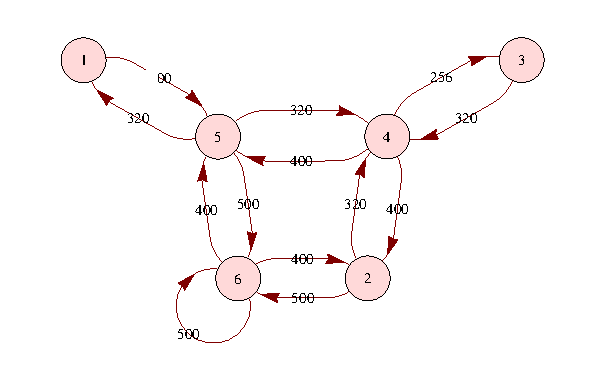
\includegraphics[scale=0.8]{slike/Q.pdf}
\frametitle{Nalaženje najkraćeg puta}
\caption{Dijagram stanja iz perspektive funkcije $Q$}
\end{figure}
}

\frame{
\frametitle{Pseudokod}
\begin{enumerate}
\item učitaj parametra $\gamma$ i matricu $R$
\item inicijaliziraj vrijednosti matrice $Q$ na 0
\item ponavljaj za svaku epizodu
	\begin{itemize}
	\item na slučajan način izaberi inicijalno stanje
	\item ponavljaj dok ne dođeš u ciljno stanje
		\begin{itemize}
		\item izaberi jedno od mogućih akcija za trenutno stanje
		\item $Q_{s, a} = R_{s, a}+\gamma \cdot \max_i\{Q_{a, a_i}\}$
		\item postavi sljedeće stanje za trenutno stanje
		\end{itemize}
	\end{itemize}
\end{enumerate}
}
\frame{
\begin{algorithmic}
\STATE učitaj parametar $\gamma$ i matricu $R$
\STATE inicijaliziraj vrijednosti matrice $Q$ na 0
\WHILE{nema konvergencije}
\STATE na slučajan način izaberi inicijalno stanje
\WHILE{nismo u završnom stanju}
\STATE izaberi jedno od mogućih akcija za trenutno stanje
\STATE $Q_{s, a} = R_{s, a}+\gamma \cdot \max_i\{Q_{a, a_i}\}$
\STATE postavi sljedeće stanje za trenutno stanje
\ENDWHILE
\ENDWHILE
\end{algorithmic}
}

\section{Implementacija i rezultati}
\frame{
\begin{center}
\begin{figure}
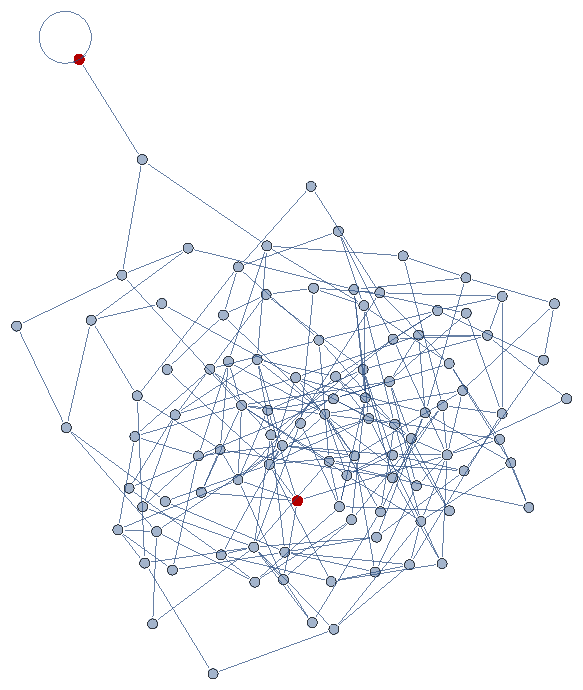
\includegraphics[scale=0.5]{slike/pokraj.pdf}
\caption{Dijagram sa 100 stanja}
\end{figure}
\end{center}
}
\frame{
\begin{center}
\begin{figure}
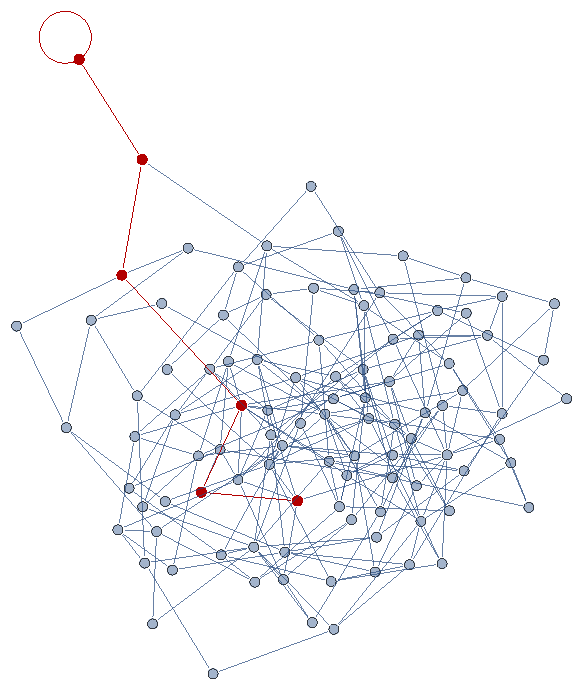
\includegraphics[scale=0.5]{slike/put.pdf}
\caption{Dijagram sa 100 stanja}
\end{figure}
\end{center}
}

\frame{
\begin{center}
\begin{figure}
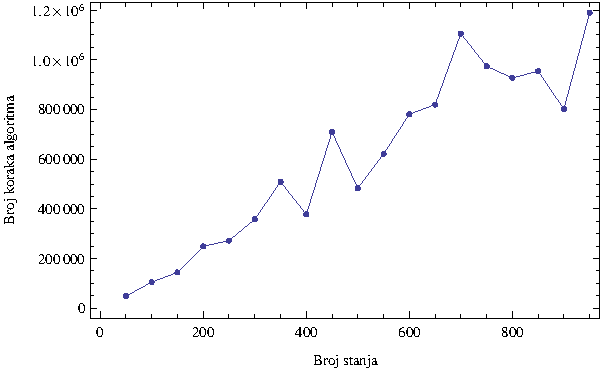
\includegraphics[scale=0.8]{slike/bench1.pdf}
\caption{Broj koraka algoritma u odnosu na broj stanja}
\end{figure}
\end{center}
}
\frame{
\begin{center}
\begin{figure}
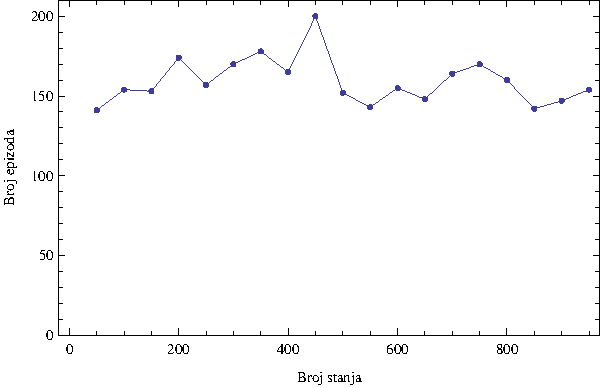
\includegraphics[scale=0.8]{slike/bench2.pdf}
\caption{Broj epizoda u odnosu na broj stanja}
\end{figure}
\end{center}
}
\frame{
\begin{center}
\begin{figure}
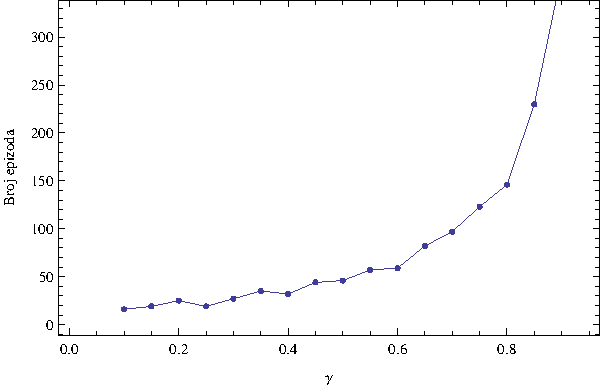
\includegraphics[scale=0.8]{slike/bench3.pdf}
\caption{Broj epizoda u odnosu na vrijednost $\gamma$}
\end{figure}
\end{center}
}
\end{document}
